


\label{programme:does}
The main steps of the programme are shortly sketched here.
The user is invited to read this Section for a better understanding
of the input, output, warning  and error messages.


\section{Preprocessing on the polygons}
\label{Preprocessing}
\begin{enumerate}
\item
The coordinates
are multiplied by \texttt{SCALE}\footnote{\label{f1}\texttt{SCALE},
\texttt{SAFE},\texttt{DISTP} and \texttt{TRANSLATE}
are constants set in the file \texttt{src/caliconfig.h}.},
a multiple of ten, and then  truncated to integers.
For example, 2.986 is considered as 2~m if \texttt{SCALE}$=1$,
and as 298~cm if \texttt{SCALE}$=100$.


\item
The landscape is relocated
so that the minimal x-coordinate (y-coordinate respect.)
is one,
\begin{itemize}
\item
 when 
a x-coordinate (y-coordinate respect.),
after multiplication by \texttt{SCALE},
is greater than 
\texttt{SAFE}$^\text{\ref{f1}}$
\item
when it is null or less than zero,
\item
 systematically when
\texttt{TRANSLATE}$^\text{\ref{f1}} = 1$.

\end{itemize}
\item
\label{supvertice}
Simplification of the polygons:
the aligned\footnote{
When the arccosinus of the angle built by 
three successive  vertices
is near to $\pi$,
 the vertices are considered as aligned and the middle one is
 suppressed.}
or too close vertices\footnote{
When the distance between two sucessive vertices is less
than or equal to \texttt{DISTP}, the second vertex is suppressed.},
 as well as the sharp spikes\footnote{
When the arccosinus of the angle built by 
three successive  vertices
is near to zero, it is supposed that
the three vertices draw a sharp spike,  and the second one is suppressed.}
are removed from the polygons.

\item
The areas and the centroids of the polygons are calculated.

\item
Convex subpolygons are created.
\end{enumerate}






\section{Steps for each pair of convex polygons}
\label{sec:steps}
For each pair of convex polygons ($P_1, P_2$), the steps are:
\begin{itemize}

\item
When  the minimal distance between the polygons $P_1$ and $P_2$ is
greater
than a given threshold, DP\footnote{\label{th}Thresholds are set in the file
\texttt{src/caliconfig.h}; they are different for each dispersal 
function. DP constants are the distances beyond which calculation
is made between centroids. DZ constants are the distances beyond which
dispersal is considered as null.},
the dispersal function is calculated between the centroids of these
polygons, and the result is multiplied by the product of their  areas.
\item
When this distance is
greater than the threshold DZ$^\text{\ref{th}}$,
the dispersal is automatically
set to zero.

\item
Otherwise, 
for each pair of convex 
subpolygons in $P_1$ and $P_2$, the \hyperlink{mink}{Minkowski sum}
  is calculated and the flow  is estimated by 
the result of an integration
on all the Minkowski sums. The integrand
is the product of the individual dispersal function
by the area of the intersection between the first subpolygon and
a translation of the second one in the pair.

\end{itemize}


\section{Integration methods}
\label{integration:methods}
Two integration
methods are implemented (See details in Section \ref{sec:integrale}):

\begin{itemize}
\item
The \textbf{grid method} :\\
Integration is made by discretisation of
 the \hyperlink{mink}{Minkowski sum} on  regular grids of
 points.
Several grids of regularly spaced points are generated,
each one randomly shifted  from the origin.
The successive results can be considered as replications.

The iterative process stops when the
number of replications is reached.


\item 
The \textbf{cubature method}:\\
This  method is a numerical adaptive cubature method over
triangles.\\
The absolute and \hyperlink{reler}{relative} precisions can be
controlled, as well as the maximal number of evaluations.


 
\end{itemize}

\section{Final results}

With the grid  method,
in addition to  the
\hyperlink{gridmean}{mean of the integrated flow}
over the replications,
the \hyperlink{gridcoefvar}{coefficient of variation} and
the \hyperlink{gridet}{standard deviation}
are calculated.

\noindent
With the cubature  method,
in addition to  the
\hyperlink{cubmean}{integrated flow},  the absolute
precision and  a
\hyperlink{cubic}{confidence interval} are calculated.

\section{The individual dispersal functions}
\label{sec:individualfunctions}
In the deliverable, some individual dispersal functions are defined.
We described here the first two ones. See  the comments in
the file \texttt{src/functions.cpp} for the subsequent ones.
These functions may be customized according to the needs.
See~paragraph~\ref{modifyfunctions}.

 The user has also the possibility
of coding the individual dispersal functions in R, but timing
performance can be affected: see the help-file
of the \verb+RCALI+ function \texttt{califlopp}.


\subsection{Individual dispersal function of oilseed rape pollen}
\label{pollen:funct}
The first function is the oilseed rape
pollen individual dispersal function
described by Étienne Klein~\cite{Klein:2006} until 50 m
and by Céline Devaux for distances beyond~50~m~\cite{Devaux:2006}:

\begin{equation}
  \label{eq:dispersion:klein}
  \phi(t)= \left\{  \begin{array}{ll}d+er+fr^2 & \textrm{when \(0\leq r\leq 1,5\)}\\
      \frac{b}{1+r^c/a} & \textrm{when \(50 \leq r < 1,5\)}\\
\text{[} \frac{b}{1+h^c/a} / (1+h)^g \text{]}  * ( 1+r)^g & \textrm{when \(r> 50\)}
\end{array}
  \right.,  r=\parallel t\parallel. 
\end{equation} 
with $a=3.80$, $b=0.03985$, $c=3.12$, $d=0.340$, $e=-0.405$,
$f=0.128$, $g=-2.29$\footnote{According to N. Colbach
  (\cite{Colbach1:2001}
and \cite{Colbach2:2001}), $g$  can vary between
$-2,14$ and $-2,56$.}, $h=50$
and with
$t$ the  distance between the source and  target points.
Distances are in meters.
See~Fig.~\ref{fig:phi:klein}.

% 
% \begin{figure}[htbp]
% \begin{center}
% 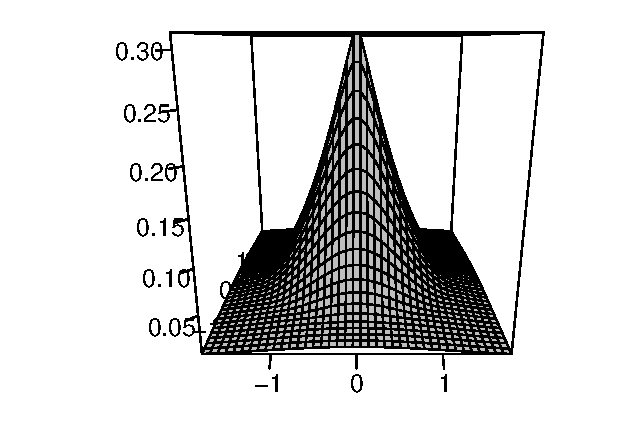
\includegraphics{./graphics/pollen.eps}
% \caption{Rape Seed Pollen Individual Dispersal Function.}
%     \label{fig:phi:klein}
% \end{center}
% \end{figure}

For this function,
the  threshold beyond which the
flow is calculated between centroids
only, is 100 m.


\medskip

\subsection{Individual dispersal function  of oilseed rape seeds}

The second function is the oilseed rape
seed individual dispersal function
proposed by Nathalie Colbach~\cite{Colbach2:2001}:
\begin{equation}
  \label{eq:dispersion:colbach}
  \phi\left(t\right)
  =
  \left\{
    \begin{array}{lll}
\dfrac{b \times c \times r^(c-2) \times \exp{ (-b \times r^c)}} {2.0*\pi}
    \end{array}
  \right.,\quad r=\left\|t\right\|.
\end{equation}
with $b = 1.38930$, $c= 2.08686$ and with
$t$ the  distance between the source  and the target points.
Distances are in meter.
See~Fig.~\ref{fig:phi:colbach}.

For this function,
the  threshold beyond which the
flow is supposed to be null is 21 m.

\begin{figure}[htbp]
  \begin{center}
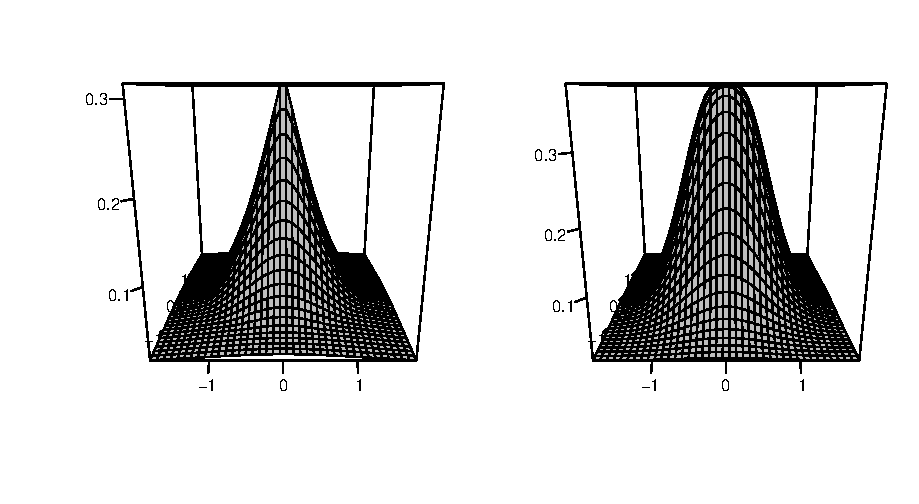
\includegraphics[width=15cm]{./VignetteDir/graphics/dispersion.eps}
%    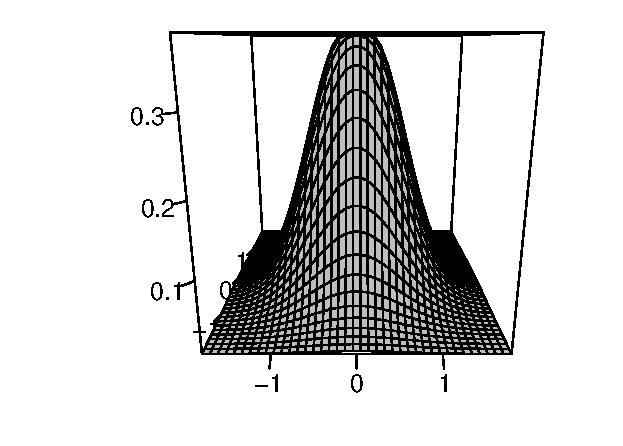
\includegraphics{./VignetteDir/graphics/seed.eps}
    \caption{Individual Dispersal Function of Pollen (on  the left) and
      Oilseed (on the right) Rape Seeds.}
     \label{fig:phi:klein}
    \label{fig:phi:colbach}
  \end{center}
\end{figure}

\subsection{How to modify or add individual dispersal functions}
\label{modifyfunctions}
The individual dispersal functions are coded in the C file
 \texttt{src/functions.cpp}.
To modify them, change the formulae expressions in the source code.
Don't forget they must be smooth functions.
Change also the DP* and DZ* constants
 in the file \texttt{src/caliconfig.h},
i.e the thresholds for  calculating dispersal between centroids only
and for considering that dispersal is zero, respectively.

In the delivered package, up to five dispersal functions 
can be defined. By default, the  DEFAULT\_NFUNCTIONS\footnote{
DEFAULT\_NFUNCTIONS is defined the file \texttt{src/caliconfig.h}.}
first functions are considered only.


After alteration of the source code, recompilation is required,
typically by using the standard R command: <tt>R CMD build RCALI</tt>
on top of your <tt>RCALI</tt> directory (see~\ref{howchanges}).
